% Options for packages loaded elsewhere
\PassOptionsToPackage{unicode}{hyperref}
\PassOptionsToPackage{hyphens}{url}
\PassOptionsToPackage{dvipsnames,svgnames,x11names}{xcolor}
%
\documentclass[
  letterpaper,
  DIV=11,
  numbers=noendperiod]{scrartcl}

\usepackage{amsmath,amssymb}
\usepackage{iftex}
\ifPDFTeX
  \usepackage[T1]{fontenc}
  \usepackage[utf8]{inputenc}
  \usepackage{textcomp} % provide euro and other symbols
\else % if luatex or xetex
  \usepackage{unicode-math}
  \defaultfontfeatures{Scale=MatchLowercase}
  \defaultfontfeatures[\rmfamily]{Ligatures=TeX,Scale=1}
\fi
\usepackage{lmodern}
\ifPDFTeX\else  
    % xetex/luatex font selection
\fi
% Use upquote if available, for straight quotes in verbatim environments
\IfFileExists{upquote.sty}{\usepackage{upquote}}{}
\IfFileExists{microtype.sty}{% use microtype if available
  \usepackage[]{microtype}
  \UseMicrotypeSet[protrusion]{basicmath} % disable protrusion for tt fonts
}{}
\makeatletter
\@ifundefined{KOMAClassName}{% if non-KOMA class
  \IfFileExists{parskip.sty}{%
    \usepackage{parskip}
  }{% else
    \setlength{\parindent}{0pt}
    \setlength{\parskip}{6pt plus 2pt minus 1pt}}
}{% if KOMA class
  \KOMAoptions{parskip=half}}
\makeatother
\usepackage{xcolor}
\setlength{\emergencystretch}{3em} % prevent overfull lines
\setcounter{secnumdepth}{-\maxdimen} % remove section numbering
% Make \paragraph and \subparagraph free-standing
\ifx\paragraph\undefined\else
  \let\oldparagraph\paragraph
  \renewcommand{\paragraph}[1]{\oldparagraph{#1}\mbox{}}
\fi
\ifx\subparagraph\undefined\else
  \let\oldsubparagraph\subparagraph
  \renewcommand{\subparagraph}[1]{\oldsubparagraph{#1}\mbox{}}
\fi


\providecommand{\tightlist}{%
  \setlength{\itemsep}{0pt}\setlength{\parskip}{0pt}}\usepackage{longtable,booktabs,array}
\usepackage{calc} % for calculating minipage widths
% Correct order of tables after \paragraph or \subparagraph
\usepackage{etoolbox}
\makeatletter
\patchcmd\longtable{\par}{\if@noskipsec\mbox{}\fi\par}{}{}
\makeatother
% Allow footnotes in longtable head/foot
\IfFileExists{footnotehyper.sty}{\usepackage{footnotehyper}}{\usepackage{footnote}}
\makesavenoteenv{longtable}
\usepackage{graphicx}
\makeatletter
\def\maxwidth{\ifdim\Gin@nat@width>\linewidth\linewidth\else\Gin@nat@width\fi}
\def\maxheight{\ifdim\Gin@nat@height>\textheight\textheight\else\Gin@nat@height\fi}
\makeatother
% Scale images if necessary, so that they will not overflow the page
% margins by default, and it is still possible to overwrite the defaults
% using explicit options in \includegraphics[width, height, ...]{}
\setkeys{Gin}{width=\maxwidth,height=\maxheight,keepaspectratio}
% Set default figure placement to htbp
\makeatletter
\def\fps@figure{htbp}
\makeatother

\KOMAoption{captions}{tableheading}
\makeatletter
\@ifpackageloaded{tcolorbox}{}{\usepackage[skins,breakable]{tcolorbox}}
\@ifpackageloaded{fontawesome5}{}{\usepackage{fontawesome5}}
\definecolor{quarto-callout-color}{HTML}{909090}
\definecolor{quarto-callout-note-color}{HTML}{0758E5}
\definecolor{quarto-callout-important-color}{HTML}{CC1914}
\definecolor{quarto-callout-warning-color}{HTML}{EB9113}
\definecolor{quarto-callout-tip-color}{HTML}{00A047}
\definecolor{quarto-callout-caution-color}{HTML}{FC5300}
\definecolor{quarto-callout-color-frame}{HTML}{acacac}
\definecolor{quarto-callout-note-color-frame}{HTML}{4582ec}
\definecolor{quarto-callout-important-color-frame}{HTML}{d9534f}
\definecolor{quarto-callout-warning-color-frame}{HTML}{f0ad4e}
\definecolor{quarto-callout-tip-color-frame}{HTML}{02b875}
\definecolor{quarto-callout-caution-color-frame}{HTML}{fd7e14}
\makeatother
\makeatletter
\@ifpackageloaded{caption}{}{\usepackage{caption}}
\AtBeginDocument{%
\ifdefined\contentsname
  \renewcommand*\contentsname{Table of contents}
\else
  \newcommand\contentsname{Table of contents}
\fi
\ifdefined\listfigurename
  \renewcommand*\listfigurename{List of Figures}
\else
  \newcommand\listfigurename{List of Figures}
\fi
\ifdefined\listtablename
  \renewcommand*\listtablename{List of Tables}
\else
  \newcommand\listtablename{List of Tables}
\fi
\ifdefined\figurename
  \renewcommand*\figurename{Figure}
\else
  \newcommand\figurename{Figure}
\fi
\ifdefined\tablename
  \renewcommand*\tablename{Table}
\else
  \newcommand\tablename{Table}
\fi
}
\@ifpackageloaded{float}{}{\usepackage{float}}
\floatstyle{ruled}
\@ifundefined{c@chapter}{\newfloat{codelisting}{h}{lop}}{\newfloat{codelisting}{h}{lop}[chapter]}
\floatname{codelisting}{Listing}
\newcommand*\listoflistings{\listof{codelisting}{List of Listings}}
\makeatother
\makeatletter
\makeatother
\makeatletter
\@ifpackageloaded{caption}{}{\usepackage{caption}}
\@ifpackageloaded{subcaption}{}{\usepackage{subcaption}}
\makeatother
\ifLuaTeX
  \usepackage{selnolig}  % disable illegal ligatures
\fi
\usepackage{bookmark}

\IfFileExists{xurl.sty}{\usepackage{xurl}}{} % add URL line breaks if available
\urlstyle{same} % disable monospaced font for URLs
\hypersetup{
  pdftitle={Examen (Partie 1)},
  colorlinks=true,
  linkcolor={blue},
  filecolor={Maroon},
  citecolor={Blue},
  urlcolor={Blue},
  pdfcreator={LaTeX via pandoc}}

\title{Examen (Partie 1)}
\author{}
\date{}

\begin{document}
\maketitle

\subsection{Questions de cours}\label{questions-de-cours}

Choisir l'unique bonne réponse:

1/ Laquelles des assertions suivantes est fausse:

\begin{enumerate}
\def\labelenumi{\alph{enumi}.}
\tightlist
\item
  la propension marginale à consommer des consommateurs est comprise
  entre 0 et 1
\item
  la consommation des consommateurs ricardiens réagit au taux d'intérêt
  réel
\item
  si tous les consommateurs sont keynésiens, une baisse du taux
  d'intérêt réel ne stimule pas la demande agrégée
\item
  la banque centrale stabilise la demande en influant sur le taux
  d'intérêt réel
\end{enumerate}

\begin{tcolorbox}[enhanced jigsaw, colbacktitle=quarto-callout-warning-color!10!white, rightrule=.15mm, left=2mm, leftrule=.75mm, colframe=quarto-callout-warning-color-frame, titlerule=0mm, colback=white, toptitle=1mm, bottomtitle=1mm, breakable, coltitle=black, title=\textcolor{quarto-callout-warning-color}{\faExclamationTriangle}\hspace{0.5em}{Correction}, bottomrule=.15mm, opacityback=0, arc=.35mm, toprule=.15mm, opacitybacktitle=0.6]

\begin{enumerate}
\def\labelenumi{\alph{enumi}.}
\tightlist
\item
  vrai (cf cours)
\item
  vrai (cf cours)
\item
  faux: même si tous les consommateurs sont ricardiens, il reste les
  entreprises qui répondent au taux d'intérêt réel
\item
  vrai (cf cours)
\end{enumerate}

\end{tcolorbox}

2/ A la suite d'un choc inconnu, on a observé une baisse de la
production accompagnée d'une augmentation de l'inflation. Après
plusieurs périodes, la production est revenue à son niveau d'origine
mais l'inflation est restée à un niveau plus haut. Quel type d'événement
est compatible avec cette observation:

\begin{enumerate}
\def\labelenumi{\alph{enumi}.}
\tightlist
\item
  Un choc négatif persistent de la production et un choc négatif
  temporaire de la demande
\item
  Un choc négatif temporaire de la production et un choc postif
  persistent de la demande
\item
  Un choc positif temporaire de la production et un choc négatif
  persistent de la demande
\item
  Un choc positif persistent de la production et un choc négatif
  temporaire de la demande
\end{enumerate}

\begin{tcolorbox}[enhanced jigsaw, colbacktitle=quarto-callout-warning-color!10!white, rightrule=.15mm, left=2mm, leftrule=.75mm, colframe=quarto-callout-warning-color-frame, titlerule=0mm, colback=white, toptitle=1mm, bottomtitle=1mm, breakable, coltitle=black, title=\textcolor{quarto-callout-warning-color}{\faExclamationTriangle}\hspace{0.5em}{Correction}, bottomrule=.15mm, opacityback=0, arc=.35mm, toprule=.15mm, opacitybacktitle=0.6]

A long terme, le production est revenue à l'équilibre donc le choc
d'offre est temporaire. L'inflation reste plus haute de manière
permanente, donc le choc sur la demande est persistent (et positif).
Comme le choc de demande est positif, pour que la production baisse à
court terme, il faut qu'il y ait en même temps un choc d'offre négatif.

\end{tcolorbox}

\subsection{Équilibre à long terme et marché du
travail.}\label{uxe9quilibre-uxe0-long-terme-et-marchuxe9-du-travail.}

On suppose que les firmes produisent avec une technologie linéaire
\(Y_t = L_t Z_t\) où \(L_t\) est le nombre d'heures travaillées, et
\(Z_t\) un choc de productivité. Le salaire horaire est \(W_t\).

1/ Quel est le coût marginal de la production?

\begin{tcolorbox}[enhanced jigsaw, colbacktitle=quarto-callout-warning-color!10!white, rightrule=.15mm, left=2mm, leftrule=.75mm, colframe=quarto-callout-warning-color-frame, titlerule=0mm, colback=white, toptitle=1mm, bottomtitle=1mm, breakable, coltitle=black, title=\textcolor{quarto-callout-warning-color}{\faExclamationTriangle}\hspace{0.5em}{Correction}, bottomrule=.15mm, opacityback=0, arc=.35mm, toprule=.15mm, opacitybacktitle=0.6]

Il faut \(\frac{Y_t}{Z_t}\) unités de travail pour produire une unité de
production. Chaque unité de travail coûte \(W_t\). Le coût (marginal)
d'une unité de production est donc \({mc}_t=\frac{Y_t}{Z_t} W_t\).

\end{tcolorbox}

Les travailleurs maximisent chaque période une fonction d'utilité
\(V(C_t,L_t) = \frac{{C_t}^{1-\sigma}}{1-\sigma} - \frac{1}{\xi}{L_t}^{\xi}\)
où \(C_t\) est la consommation et \(L_t\) le nombre d'heures travaillées
et \(\xi\) un paramètre positif. On note \(P_t\) le niveau des prix.

2/ Écrire la contrainte de budget intratemporelle des travailleurs et
déterminer leur offre de travail à l'équilibre.

\begin{tcolorbox}[enhanced jigsaw, colbacktitle=quarto-callout-warning-color!10!white, rightrule=.15mm, left=2mm, leftrule=.75mm, colframe=quarto-callout-warning-color-frame, titlerule=0mm, colback=white, toptitle=1mm, bottomtitle=1mm, breakable, coltitle=black, title=\textcolor{quarto-callout-warning-color}{\faExclamationTriangle}\hspace{0.5em}{Correction}, bottomrule=.15mm, opacityback=0, arc=.35mm, toprule=.15mm, opacitybacktitle=0.6]

Contrainte de budget: \(P_t C_t \leq W_t L_t\). En maximisant la
fonction d'utilité sous la contrainte de budget on obtient:
\(L_t = \left(\frac{W_t}{P_t}\right)^{\xi}\).

\end{tcolorbox}

3/ Quel est l'équilibre sur le marché du travail? Représentation
graphique.

\begin{tcolorbox}[enhanced jigsaw, colbacktitle=quarto-callout-warning-color!10!white, rightrule=.15mm, left=2mm, leftrule=.75mm, colframe=quarto-callout-warning-color-frame, titlerule=0mm, colback=white, toptitle=1mm, bottomtitle=1mm, breakable, coltitle=black, title=\textcolor{quarto-callout-warning-color}{\faExclamationTriangle}\hspace{0.5em}{Correction}, bottomrule=.15mm, opacityback=0, arc=.35mm, toprule=.15mm, opacitybacktitle=0.6]

L'offre de travail vient d'être calculée:
\(L^S_t = \left(\frac{W_t}{P_t}\right)^{\xi}\).

La demande de travail vient de la fonction de production et vaut:
\(L^D_t = \frac{Y_t}{Z_t}\).

A l'équilibre on a \(L^D_t = L^S_t\) donc
\(\left(\frac{W_t}{P_t}\right)^{\xi} = \frac{Y_t}{Z_t}\)

\begin{figure}[H]

{\centering 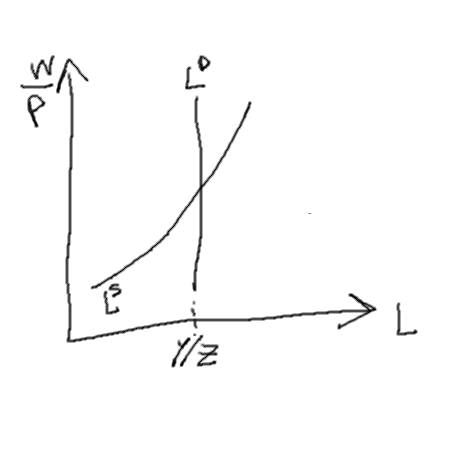
\includegraphics{labour.png}

}

\caption{Marché du travail}

\end{figure}%

\end{tcolorbox}

On suppose maintenant que les firmes fixent leur prix optimal
\(P^{\star}_t\) en intégrant une marge \(\mu\) sur le coût marginal.

4/ En supposant les prix parfaitement flexibles calculer l'équilibre de
long terme pour les différentes variables macroéconomiques. Commenter
l'effet de la productivité \(Z\) et du taux de marge \(\mu\) sur \(Y\)
et \(L\).

\begin{tcolorbox}[enhanced jigsaw, colbacktitle=quarto-callout-warning-color!10!white, rightrule=.15mm, left=2mm, leftrule=.75mm, colframe=quarto-callout-warning-color-frame, titlerule=0mm, colback=white, toptitle=1mm, bottomtitle=1mm, breakable, coltitle=black, title=\textcolor{quarto-callout-warning-color}{\faExclamationTriangle}\hspace{0.5em}{Correction}, bottomrule=.15mm, opacityback=0, arc=.35mm, toprule=.15mm, opacitybacktitle=0.6]

Le prix optimal des firmes s'écrit simplement:

\[P^{\star}_t = mc_t (1+\mu) = \frac{Y_t}{Z_t} W_t (1+\mu)\]

Lorsque les prix sont flexibles, toutes les firmes fixent le même prix
qui est donc égal à l'indice des prix: \(P^{\star}_t = P_t\)

On a donc:

\[\frac{P_t}{W_t} = \left( \frac{Y_t}{Z_t} \right)^{-\frac{1}{\xi}} = \frac{Y_t}{Z_t} (1+\mu)\]

Et: \[Y_t = Z_t (1+\mu)^{-(1+\frac{1}{\xi})}\]

\[L_t = (1+\mu)^{-(1+\frac{1}{\xi})}\]

Commentaires:

\begin{itemize}
\item
  La production d'équilibre et l'emploi sont négativement affectée par
  la marge. C'est logique car les firmes en compétition monopolistique
  raréfient les produits de sorte à augmenter les prix et les profits.
\item
  Une augmentation de la productivité augmente la production comme
  attendu.
\item
  Une augmentation de la productivité n'a pas d'effet sur l'emploi dans
  ce modèle. Comme on a \(L_t \frac{W_t}{P_t} = C_t\) et que la
  consommation augmente, on voit que la hausse de salaire réel décourage
  les travailleurs d'augmenter leur offre d'emploi. Cet effet précis,
  que l'on observe à l'equilibre serait différent pour une autre
  spécification de l'utilité des travailleurs.
\end{itemize}

\end{tcolorbox}

\subsection{Principe de Taylor}\label{principe-de-taylor}

On considère ici une économie loglinéarisée caractérisée par les courbes
IS et PC suivantes:

\begin{equation}\phantomsection\label{eq-is}{y_t = y_{t+1} - \sigma \left( i_t - \pi_{t+1} \right) + e^{\pi}_t}\end{equation}
\begin{equation}\phantomsection\label{eq-pc}{\pi_t = \kappa (y_t - e^y_t)  + \beta \pi_{t+1}}\end{equation}

où \(\pi_t\) dénote l'inflation, \(y_t\) la production, \(i_t\) le taux
d'intérêt et où \(\sigma\) et \(\kappa\) sont des paramètres réels
positifs et où \(\beta \in ]0,1[\) est le facteur d'escompte.

Les variables \(e^{\pi}_t\) et \(e^{y}_t\) sont respectivement des chocs
de demande et d'offre.\footnote{Ici, la courbe de Philips provient de la
  fixation des prix par des entreprises en compétitions monopolistiques,
  qui optimisent leur profits futurs plutôt qu'instantané. On parle de
  courbe de Philips augmentée par les anticipations.}. Ils sont pris
comme exogènes et on les suppose bornés. On suppose qu'il n'y a pas
d'incertitude sur la valeur des chocs futurs, de sorte qu'on peut
omettre les symboles d'espérance et considérer toutes leurs valeurs
comme connues.

La banque centrale suit une règle pour fixer son taux d'intérêt:
\begin{equation}\phantomsection\label{eq-taylor}{i_t = i^{\star} + \varphi_y (y_t - e^{\pi}_t) + \varphi_\pi (\pi_t - \pi^{\star})}\end{equation}

avec la cible d'inflation égale au taux d'intérêt cible:
\(i^{\star}=\pi^{\star}\).

On dit qu'une règle de Taylor satisfait le principe de Taylor, si en
réponse à un choc de demande permanent ayant pour effet d'augmenter
l'inflation d'1\%, la banque centrale augmente le taux d'intérêt de plus
d'1\%.

\begin{enumerate}
\def\labelenumi{\arabic{enumi}.}
\tightlist
\item
  Définir deux matrices A, B telles que:
\end{enumerate}

\[z_{t+1} = A z_t + B e_t\]

où \(z_t=(\pi_t, y_t)\) et \(e_t = (e^{\pi}_t, e^{y}_t)\)

\begin{enumerate}
\def\labelenumi{\arabic{enumi}.}
\setcounter{enumi}{1}
\tightlist
\item
  Montrer que les niveaux d'inflation et de production sont uniquement
  déterminés à toutes les dates \(t\geq 0\) si
  \[\varphi_{\pi} + \frac{1-\beta}{\kappa} \varphi_{y}> 1\] Cela
  correspond-il a une banque centrale plus active ou plus passive
  vis-à-vis de l'inflation? Comparer avec le principe de Taylor.
\end{enumerate}

\begin{tcolorbox}[enhanced jigsaw, colbacktitle=quarto-callout-warning-color!10!white, rightrule=.15mm, left=2mm, leftrule=.75mm, colframe=quarto-callout-warning-color-frame, titlerule=0mm, colback=white, toptitle=1mm, bottomtitle=1mm, breakable, coltitle=black, title=\textcolor{quarto-callout-warning-color}{\faExclamationTriangle}\hspace{0.5em}{Correction}, bottomrule=.15mm, opacityback=0, arc=.35mm, toprule=.15mm, opacitybacktitle=0.6]

Si A n'est pas inversible, pour une valeur \(z_{t+1}\) donnée il peut
exister plusieurs valeurs de \(z_t\).

On suppose donc que \(A\) est inversible on peut alors écrire

\[z_t = A^{-1} z_{t+1} -  A^{-1} B e_{t+k}\] d'où l'on déduit
formellement:

\[z_t = -\sum_{k \geq 0} \left(A^{-1}\right)^k (A^{-1} B) e_{t+k}\].

Pour que cette somme ne diverge pour aucune valeur de
\((e_{t+k})_{k\geq0}\) il faut que le rayon spectral de \(A^{-1}\) soit
plus petit que 1, donc que toutes les valeurs propres de \(A\) soient
supérieures à 1. En calculant les deux valeurs propres on trouve la
condition:

\[\varphi_{\pi} + \frac{1-\beta}{\kappa} \varphi_{y}> 1\]

Pour que cette condition soit satisfaite, il faut que \(\varphi_{\pi}\)
soit suffisament grand.

On peut interpréter ce résultat en disant que la banque centrale doit
réagir suffisament à l'inflation anticipée pour que l'inflation
ajourd'hui soit bien définie.

D'après l'équation (2), un choc de demande permanent qui augmente
l'inflation de \(\Delta \pi=1\%\) augmente la production de
\(\Delta y=\frac{1-\beta}{\kappa}\Delta \pi\). En suivant la règle de
l'énoncé la réaction de la banque centrale est donc:

\[\Delta i = \varphi_{\pi} \Delta \pi + \varphi{y} \Delta y = \left( \varphi_{\pi}  +\frac{1-\beta}{\kappa}  \varphi_y \right)\Delta \pi\]

Le critère de Taylor se confond donc dans ce cas précis avec un critère
de détermination.

\end{tcolorbox}



\end{document}
